\begin{figure}[htp]
            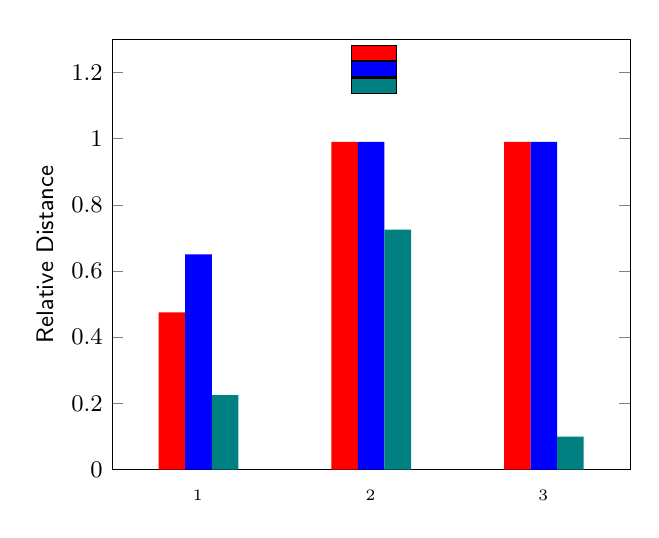
\begin{tikzpicture}[scale=0.96]
            [every plot/.append style={}]
            \begin{axis}[
                major x tick style = transparent,
                ybar=0*\pgflinewidth,
                bar width=10pt,
%                ymode = log,
%                log origin=infty,
                ylabel = {\small \textsf{Relative Distance}},
                yticklabel style = {font=\small},        
                xticklabel style = {font=\small},
                symbolic x coords={{\fact}$_1$,{\fact}$_2$,{\fact}$_3$},
                xtick=data,
                scaled y ticks = false,
                enlarge x limits=0.25,
                ymin=0,
                ymax=1.3,
                legend cell align=left,
                legend style={
                    column sep=0.6ex,
                    legend columns = 1,
                    draw = none,
                    fill = none,
                    at={(0.6,1)},
                    font=\scriptsize,
                    }
                ]
                        
                \addplot [area legend,draw=none,fill=red]
                coordinates {({\fact}$_1$, 0.475)({\fact}$_2$,0.99) ({\fact}$_3$,0.99) };
                
                \addplot [area legend,draw=none,fill=blue]
                coordinates {({\fact}$_1$,0.65)({\fact}$_2$, 0.99) ({\fact}$_3$,0.99) };
                
                \addplot [area legend,draw=none,fill=teal]
                coordinates {({\fact}$_1$,0.225)({\fact}$_2$, 0.725) ({\fact}$_3$,0.1)};
                
                \legend{\textsf{{\aggravation}}, \textsf{{\intervention}}, \textsf{{\solution}}}
            \end{axis}
        \end{tikzpicture}
    \caption{\small Relative Distance}
    \label{fig:kfolds}
\end{figure}